\clearpage
\subsubsection{Strukturplan}
\label{subsubsec:Strukturplan_Atmega}

In Abbildung \ref{fig:Softwareuebersicht_Atmega2560} wird aufgezeicht, wie die Software aufgebaut ist, und welcher Teil der Software von welchen Libraries abhängig ist. Wie in Kapitel \ref{sec:Software_Atmega2560} beschrieben kann die Software in folgende Teile gegliedert werden:
\begin{itemize}
\item Init/Main
\item User Application
\item API - Application-Programming-Interface
\item HAL - Hardware-Abstraction-Layer
\item Interfaces / Pins
\end{itemize}

\begin{figure}[h!]
	\centering
	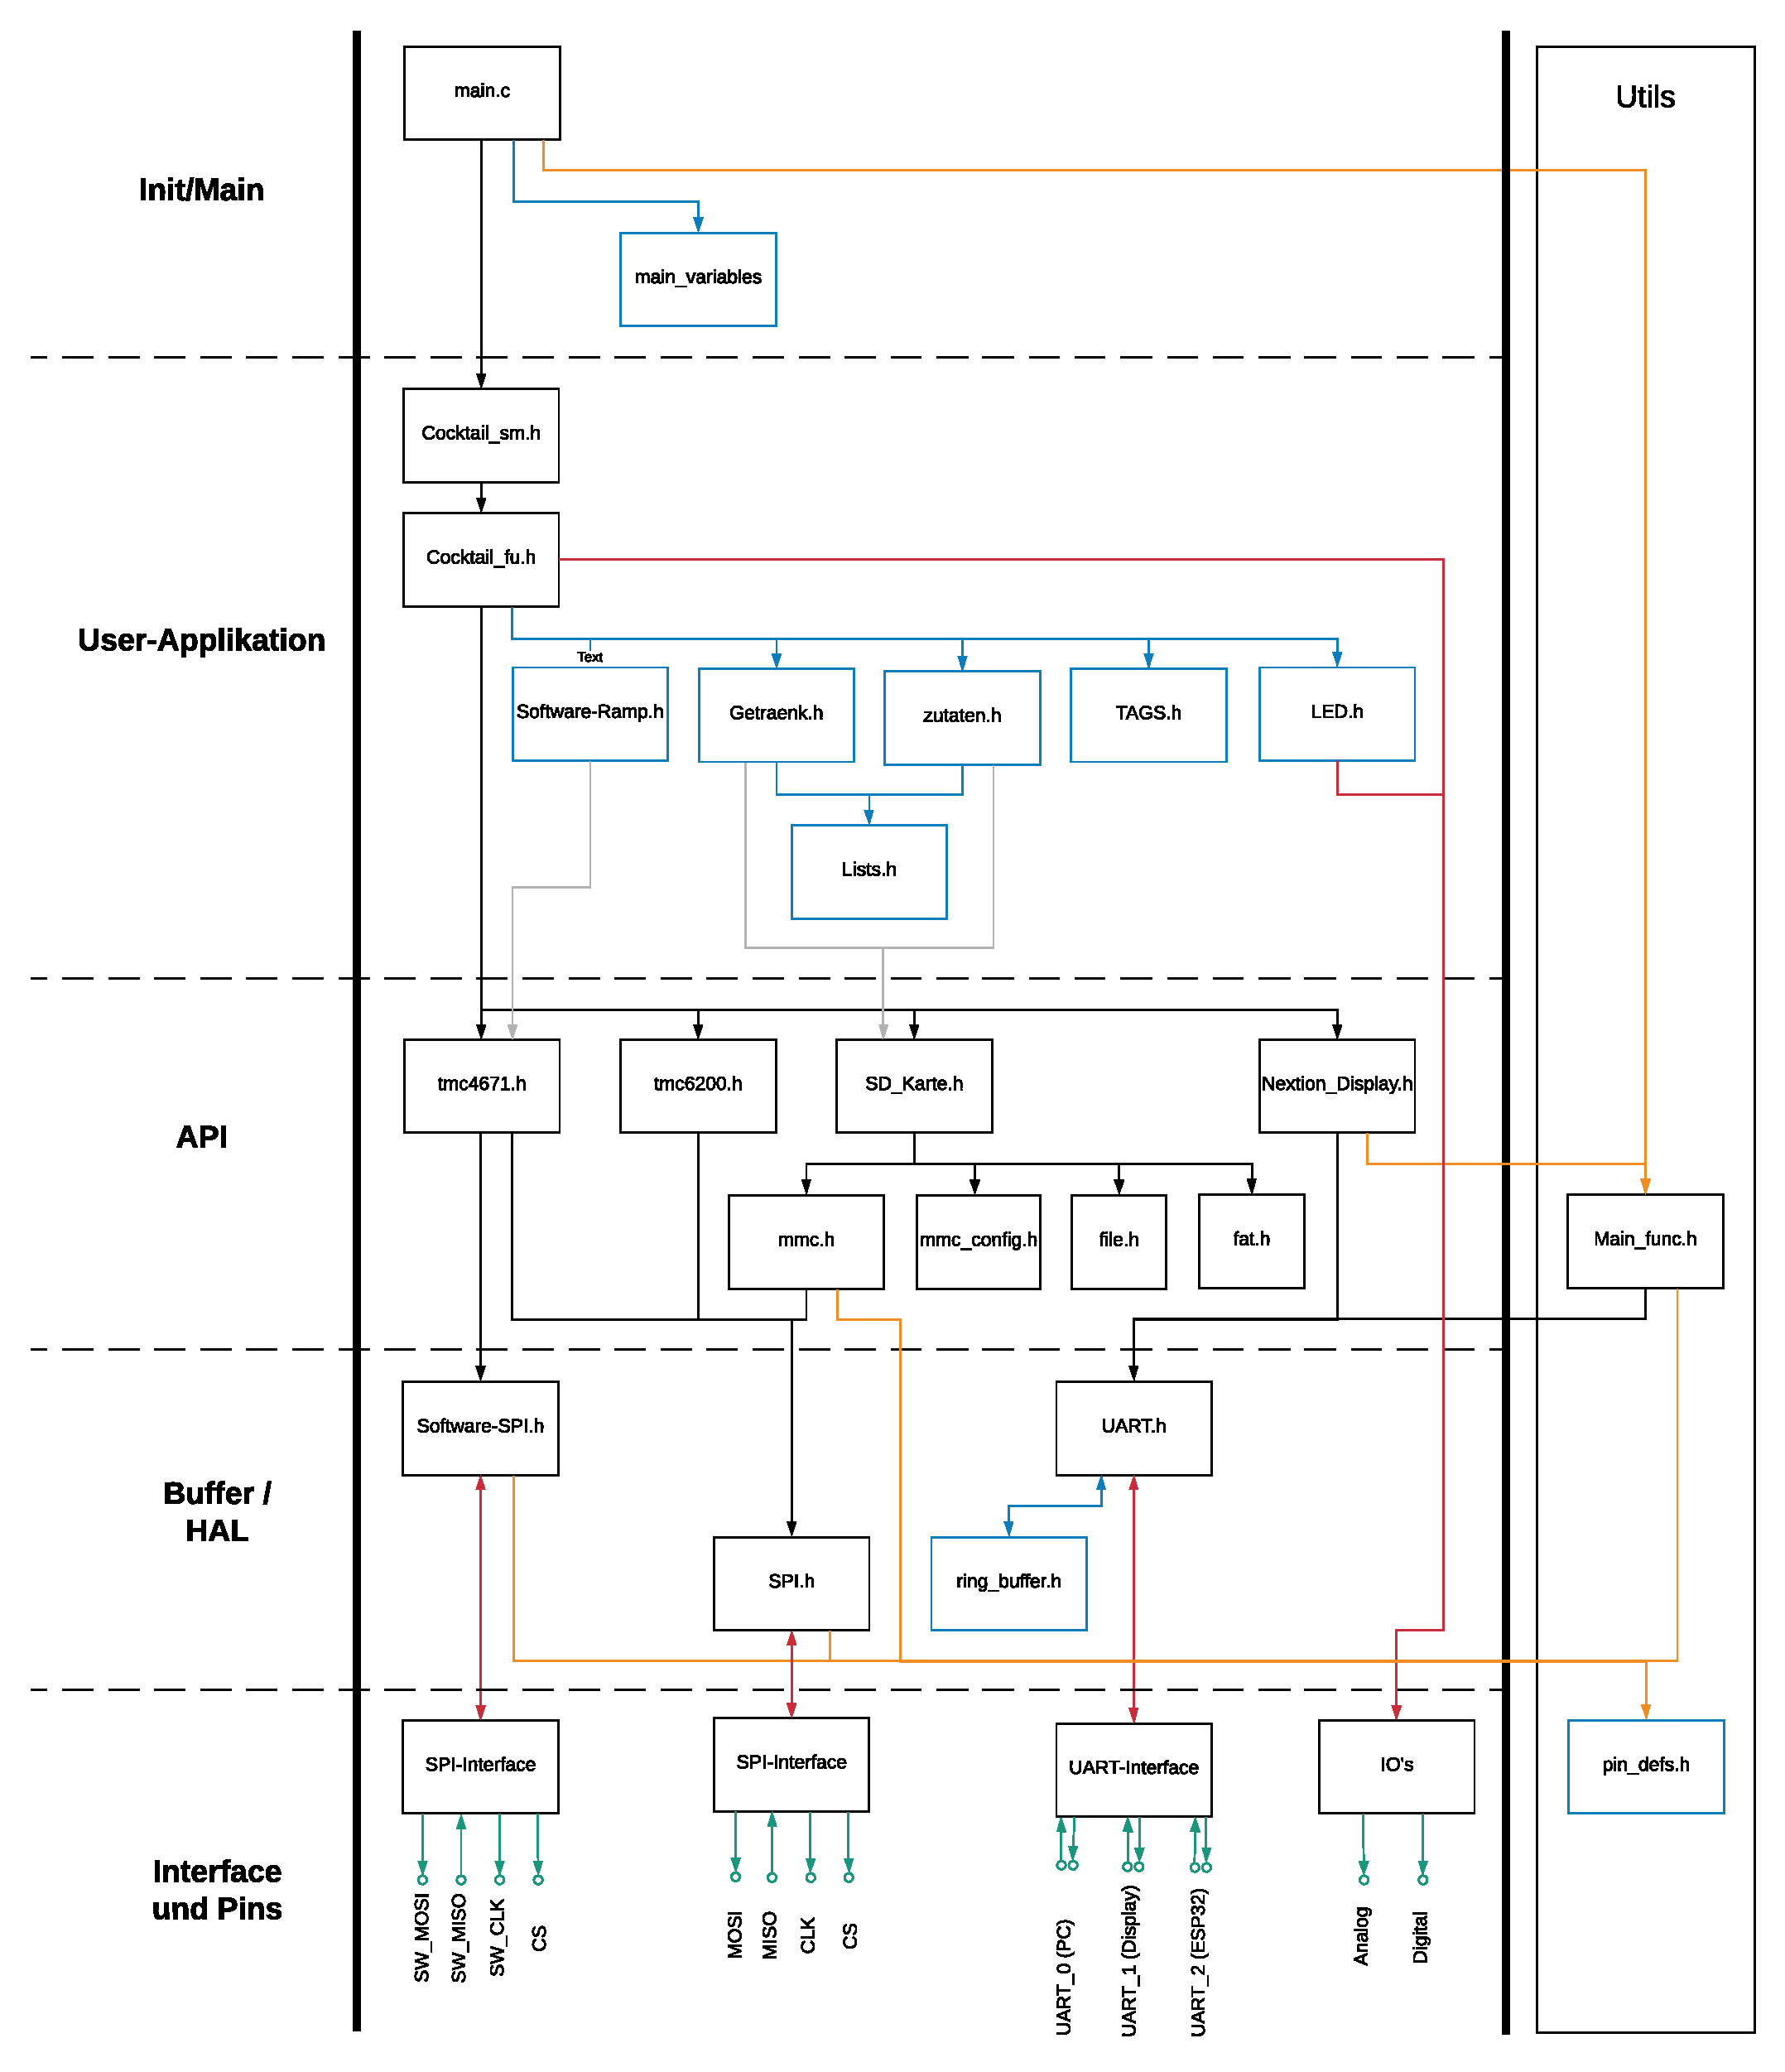
\includegraphics[width=\textwidth]{graphics/Softwareuebersicht.pdf}
	\caption{Softwareübersicht Atmega2560.}
	\label{fig:Softwareuebersicht_Atmega2560}
\end{figure}

